\documentclass[11pt]{article}
\usepackage[margin=1in]{geometry}
\usepackage{amsmath, amssymb, amsthm}
\usepackage{tikz}
\usepackage{mdframed}
\usepackage{booktabs}

% Define custom environments for a professional notebook layout
\newtheorem{problem}{Problem}
\newtheorem{theorem}{Theorem}
\newtheorem{definition}{Definition}

\title{\vspace{-2cm}\textbf{Algebraic Curve Theory \& Codes}}
\author{Riemann Surfaces \& Winding Forms}
\date{}

\begin{document}
	
	\maketitle
	\thispagestyle{empty} % Keeps the page clean for a one-problem-per-page layout
	
	\begin{problem}
		Prove that a classical Goppa code $C \subseteq \mathbb{F}_q^n$ is mathematically well-defined as the kernel of a linear map by representing the codewords as integrals of meromorphic winding forms on the Riemann sphere $\mathbb{P}^1$.
	\end{problem}
	
	\vspace{0.5cm}
	
	\begin{mdframed}[backgroundcolor=gray!5, linecolor=gray!50, linewidth=1pt]
		\textbf{Conceptual Proof \& Geometric Translation:}
		
		\vspace{0.3cm}
		\textbf{1. The Codeword as a Winding Form} \\
		Let $L = \{a_1, a_2, \dots, a_n\}$ be the support set. We lift the discrete code vector $c = (c_1, \dots, c_n)$ into a continuous meromorphic differential form $\omega_c$ on the complex projective line $\mathbb{P}^1(\mathbb{C})$. We define this as a sum of local winding forms scaled by the coordinates:
		$$ \omega_c = \sum_{i=1}^n c_i \frac{dz}{z - a_i} $$
		
		\vspace{0.2cm}
		\textbf{2. The Extraction Operator (Linear Subspace)} \\
		To recover the coordinate $c_j$, we apply the Cauchy Integral Formula along a closed contour $\gamma_j$ enclosing only the pole at $a_j$:
		$$ c_j = \frac{1}{2\pi i} \oint_{\gamma_j} \omega_c $$
		Because the contour integral is a linear operator, the set of all valid coordinate vectors extracted from these forms inherits the structure of a well-defined linear subspace.
		
		\vspace{0.5cm}
		% TikZ Placeholder for Visualizing the Riemann Sphere and Contours
		\begin{center}
			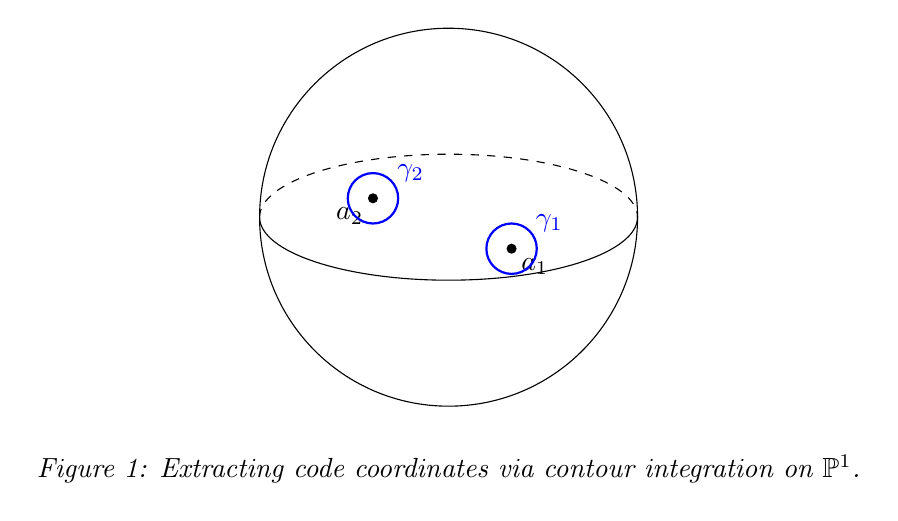
\begin{tikzpicture}[scale=0.8]
				% TODO: Draw the Riemann sphere (genus 0 surface)
				\draw (0,0) circle (3cm);
				\draw[dashed] (-3,0) arc (180:0:3cm and 1cm);
				\draw (-3,0) arc (180:360:3cm and 1cm);
				
				% TODO: Plot poles a_i and draw local oriented winding contours \gamma_i around them
				\filldraw (1,-0.5) circle (2pt) node[below right] {$a_1$};
				\draw[->, thick, blue] (1,-0.5) circle (0.4cm);
				\node[blue] at (1.6,-0.1) {$\gamma_1$};
				
				\filldraw (-1.2,0.3) circle (2pt) node[below left] {$a_2$};
				\draw[->, thick, blue] (-1.2,0.3) circle (0.4cm);
				\node[blue] at (-0.6,0.7) {$\gamma_2$};
				
				\node at (0, -4) {\textit{Figure 1: Extracting code coordinates via contour integration on $\mathbb{P}^1$.}};
			\end{tikzpicture}
		\end{center}
		\vspace{0.5cm}
		
		\textbf{3. The Goppa Constraint and the Kernel} \\
		Let $g(z)$ be the Goppa polynomial of degree $t$. We constrain $\omega_c$ such that it must be identically zero at the roots of $g(z)$. This constraint translates to multiplying $\omega_c$ by a holomorphic test function $h(z)$ of degree less than $t$, yielding a new closed form $\eta = h(z)\omega_c$.
		
		By the Generalized Stokes' Theorem (Global Residue Theorem) on the compact Riemann manifold $M = \mathbb{P}^1 \setminus \{a_1, \dots, a_n\}$, the sum of the boundary integrals must vanish:
		$$ \sum_{i=1}^n \frac{1}{2\pi i} \oint_{\gamma_i} h(z) \omega_c = 0 \implies \sum_{i=1}^n c_i h(a_i) = 0 $$
		By iterating through a basis of test polynomials for $h(z)$, we generate exactly $t$ independent linear parity-check equations. Therefore, the Goppa code is rigorously well-defined as the kernel of these integral constraints.
	\end{mdframed}

	\newpage
	
	\begin{problem}
		Consider an Algebraic Geometry (AG) differential code $C_\Omega(D, G)$ constructed on an elliptic curve $E$ over $\mathbb{F}_q$. 
		\begin{itemize}
			\item[(a)] Apply the Riemann-Roch Theorem to derive the bounds for the dimension $k$ and minimum distance $d$, demonstrating the "genus penalty."
			\item[(b)] Use the Hasse-Weil bound to explain why moving to a genus-$1$ curve allows for longer codes than the classical projective line $\mathbb{P}^1$, using $E/\mathbb{F}_{16}$ as a concrete example.
		\end{itemize}
	\end{problem}
	
	\vspace{0.5cm}
	
	\begin{mdframed}[backgroundcolor=gray!5, linecolor=gray!50, linewidth=1pt]
		\textbf{Solution:}
		
		\vspace{0.3cm}
		\textbf{Part (a): The Riemann-Roch Theorem and Genus $1$} \\
		Let $E$ be an elliptic curve, which is a Riemann surface of genus $g = 1$. Let $D = P_1 + P_2 + \dots + P_n$ be the support divisor and $G$ be the divisor of zeroes, with $\text{supp}(D) \cap \text{supp}(G) = \emptyset$. 
		
		The code $C_\Omega(D, G)$ is defined as the image of the residue map on the space of differentials $\Omega(G - D)$. By the Riemann-Roch theorem:
		$$l(A) - l(K - A) = \deg(A) + 1 - g$$
		For $g=1$, the dimension of the code is mathematically bounded by:
		$$k \geq n - \deg(G) + g - 1 \implies k \geq n - \deg(G)$$
		The minimum designed distance is bounded by:
		$$d \geq \deg(G) - (2g - 2) \implies d \geq \deg(G)$$
		Compared to a rational curve on $\mathbb{P}^1$ ($g=0$), the topological "hole" of the torus reduces our design parameters by exactly $1$. This reduction in minimum distance or dimension is known as the genus penalty.
		
		\vspace{0.5cm}
		% TikZ Placeholder: Elliptic Curve as a Flat Torus
		\begin{center}
			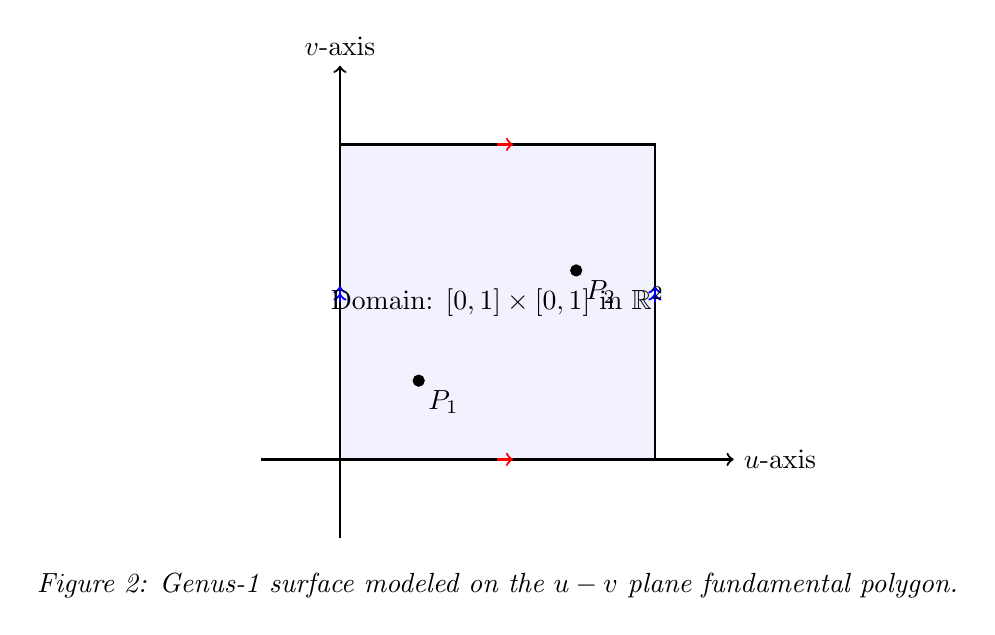
\begin{tikzpicture}[scale=2]
				% Visualizing the genus-1 surface using the 2D domain in R^2
				\draw[thick, fill=blue!5] (0,0) rectangle (2,2);
				
				% u-axis and v-axis
				\draw[->, thick] (-0.5,0) -- (2.5,0) node[right] {$u$-axis};
				\draw[->, thick] (0,-0.5) -- (0,2.5) node[above] {$v$-axis};
				
				% Edge identifications to create the Torus topology
				\draw[->, thick, red] (1,0) -- (1.1,0);
				\draw[->, thick, red] (1,2) -- (1.1,2);
				
				\draw[->>, thick, blue] (2,1) -- (2,1.1);
				\draw[->>, thick, blue] (0,1) -- (0,1.1);
				
				\node at (1,1) {Domain: $[0,1] \times [0,1]$ in $\mathbb{R}^2$};
				
				% Plotting Support Points
				\filldraw (0.5, 0.5) circle (1pt) node[below right] {$P_1$};
				\filldraw (1.5, 1.2) circle (1pt) node[below right] {$P_2$};
				
				\node at (1, -0.8) {\textit{Figure 2: Genus-1 surface modeled on the $u-v$ plane fundamental polygon.}};
			\end{tikzpicture}
		\end{center}
		\vspace{0.5cm}
		
		\textbf{Part (b): The Hasse-Weil Bound Advantage} \\
		On the projective line $\mathbb{P}^1(\mathbb{F}_{16})$, the maximum number of rational points available to form the support divisor $D$ is bounded strictly by $q + 1 = 17$. Thus, classical codes are rigidly bounded to length $n \leq 17$.
		
		However, the number of rational points on an elliptic curve $E(\mathbb{F}_q)$ is governed by Hasse's Theorem:
		$$|E(\mathbb{F}_q)| \leq q + 1 + 2\sqrt{q}$$
		For the field $\mathbb{F}_{16}$, we have $q=16$. Evaluating the theoretical upper bound:
		$$|E(\mathbb{F}_{16})| \leq 16 + 1 + 2\sqrt{16} = 17 + 8 = 25$$
		By accepting the genus penalty of $g=1$, the algebraic geometry framework allows the maximum code length to expand from $n=17$ to $n=25$, demonstrating the fundamental tradeoff in AG coding theory.
	\end{mdframed}

	\newpage
	\begin{problem}
		Let $E$ be the elliptic curve defined by the affine equation $y^2 + y = x^3 + x$ over the finite field $\mathbb{F}_4$. Let $P_\infty$ be the single point at infinity. 
		\begin{itemize}
			\item[(a)] Using the Riemann-Roch Theorem, determine the dimension $l(mP_\infty)$ for $m \in \{1, 2, 3, 4\}$.
			\item[(b)] Construct the explicit basis for the vector spaces $L(mP_\infty)$ for each $m$, using the rational coordinate functions $x$ and $y$.
		\end{itemize}
	\end{problem}
	
	\vspace{0.5cm}
	
	\begin{mdframed}[backgroundcolor=gray!5, linecolor=gray!50, linewidth=1pt]
		\textbf{Solution:}
		
		\vspace{0.3cm}
		\textbf{Part (a): Dimensions via Riemann-Roch} \\
		The curve $E$ is an elliptic curve, meaning its genus is $g = 1$. The Riemann-Roch theorem states that for a divisor $A$ with $\deg(A) > 2g - 2$, the dimension of the function space is exactly:
		$$l(A) = \deg(A) + 1 - g$$
		Since $2(1) - 2 = 0$, this simplified formula applies for all $m \geq 1$. Therefore, for the divisor $A = mP_\infty$, we have $l(mP_\infty) = m$.
		\begin{itemize}
			\item $l(P_\infty) = 1$
			\item $l(2P_\infty) = 2$
			\item $l(3P_\infty) = 3$
			\item $l(4P_\infty) = 4$
		\end{itemize}
		
		\vspace{0.3cm}
		\textbf{Part (b): Constructing the Explicit Bases} \\
		The space $L(mP_\infty)$ consists of all rational functions on $E$ that have no poles anywhere except possibly at $P_\infty$, and the pole at $P_\infty$ can be of order at most $m$.
		
		We analyze the pole orders of the affine coordinate functions $x$ and $y$ at $P_\infty$:
		\begin{itemize}
			\item The function $x$ has a pole of order $2$ at $P_\infty$. Thus, $x \in L(2P_\infty)$.
			\item The function $y$ has a pole of order $3$ at $P_\infty$. Thus, $y \in L(3P_\infty)$.
		\end{itemize}
		
		We build the bases iteratively by finding combinations of $x$ and $y$ that satisfy the allowed pole orders:
		
		\textbf{1. Space $L(P_\infty)$:} 
		The dimension is $1$. The only functions with no poles (or a pole of order 0) are the constants.
		$$ \text{Basis for } L(P_\infty) = \{ 1 \} $$
		
		\textbf{2. Space $L(2P_\infty)$:} 
		The dimension is $2$. We need a function with a pole of order $2$, which is $x$.
		$$ \text{Basis for } L(2P_\infty) = \{ 1, x \} $$
		
		\textbf{3. Space $L(3P_\infty)$:} 
		The dimension is $3$. We need a function with a pole of order $3$, which is $y$.
		$$ \text{Basis for } L(3P_\infty) = \{ 1, x, y \} $$
		
		\textbf{4. Space $L(4P_\infty)$:} 
		The dimension is $4$. We need a function with a pole of order $4$. Since $x$ has a pole of order $2$, the function $x^2$ has a pole of order $4$.
		$$ \text{Basis for } L(4P_\infty) = \{ 1, x, y, x^2 \} $$
		
		\vspace{0.5cm}
		% TikZ Placeholder: Table of rational functions evaluated at support points
		\begin{center}
			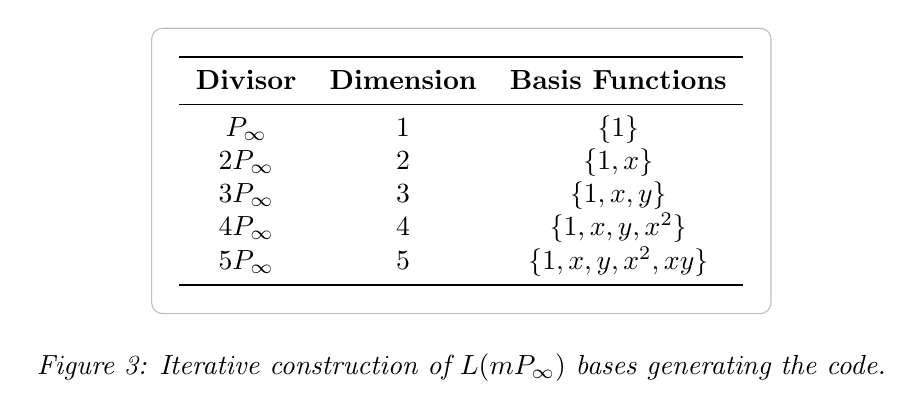
\begin{tikzpicture}
				\node[draw=gray!50, fill=white, inner sep=10pt, rounded corners] {
					\begin{tabular}{c c c}
						\toprule
						\textbf{Divisor} & \textbf{Dimension} & \textbf{Basis Functions} \\
						\midrule
						$P_\infty$  & 1 & $\{1\}$ \\
						$2P_\infty$ & 2 & $\{1, x\}$ \\
						$3P_\infty$ & 3 & $\{1, x, y\}$ \\
						$4P_\infty$ & 4 & $\{1, x, y, x^2\}$ \\
						$5P_\infty$ & 5 & $\{1, x, y, x^2, xy\}$ \\
						\bottomrule
					\end{tabular}
				};
				\node at (0, -2.5) {\textit{Figure 3: Iterative construction of $L(mP_\infty)$ bases generating the code.}};
			\end{tikzpicture}
		\end{center}
		
		\vspace{0.2cm}
		\textbf{Connection to AG Codes:} \\
		To construct the generator matrix $G$ for an algebraic geometry code of dimension $k=4$, we would take the 4 basis functions $\{1, x, y, x^2\}$ and evaluate them at the chosen support points $P_1, \dots, P_n$ on the curve. Each evaluated function forms one row of the matrix $G$.
	\end{mdframed}

	\newpage
	\begin{problem}
		Let $E$ be the elliptic curve $y^2 + y = x^3 + x$ over $\mathbb{F}_4$. Let the support divisor $D = P_1 + P_2 + P_3 + P_4$ consist of all affine rational points on $E(\mathbb{F}_4)$, and let $G = 3P_\infty$ be the constraint divisor. 
		
		Using the Riemann-Roch basis $\{1, x, y\}$ derived for $L(3P_\infty)$, construct the exact generator matrix $G_{AG}$ for the algebraic geometry code $C_L(D, G)$.
	\end{problem}
	
	\vspace{0.5cm}
	
	\begin{mdframed}[backgroundcolor=gray!5, linecolor=gray!50, linewidth=1pt]
		\textbf{Solution:}
		
		\vspace{0.3cm}
		\textbf{Step 1: Find the rational points of $E(\mathbb{F}_4)$} \\
		The field $\mathbb{F}_4$ consists of the elements $\{0, 1, \alpha, \alpha^2\}$ where $\alpha^2 + \alpha + 1 = 0$. Note that in characteristic 2, addition and subtraction are identical. For any $y \in \mathbb{F}_4$, the expression $y^2 + y$ evaluates to either $0$ (if $y \in \{0, 1\}$) or $1$ (if $y \in \{\alpha, \alpha^2\}$). 
		
		We evaluate $x^3 + x$ for each $x \in \mathbb{F}_4$ to find valid coordinates:
		\begin{itemize}
			\item Let $x = 0$: $x^3 + x = 0$. We need $y^2 + y = 0$, giving $y \in \{0, 1\}$. 
			\\ Points: $P_1 = (0,0), P_2 = (0,1)$.
			\item Let $x = 1$: $x^3 + x = 1 + 1 = 0$. We need $y^2 + y = 0$, giving $y \in \{0, 1\}$. 
			\\ Points: $P_3 = (1,0), P_4 = (1,1)$.
			\item Let $x = \alpha$: $x^3 + x = \alpha^3 + \alpha = 1 + \alpha = \alpha^2$. We need $y^2 + y = \alpha^2$. Since $y^2 + y \in \{0, 1\}$ for all $y \in \mathbb{F}_4$, there are no solutions.
			\item Let $x = \alpha^2$: $x^3 + x = (\alpha^2)^3 + \alpha^2 = 1 + \alpha^2 = \alpha$. No solutions.
		\end{itemize}
		Our support points are strictly $P_1(0,0), P_2(0,1), P_3(1,0), P_4(1,1)$.
		
		\vspace{0.3cm}
		\textbf{Step 2: Evaluate the basis functions at the support} \\
		The code $C_L(D, G)$ is formed by evaluating every function $f \in L(3P_\infty)$ at the points in $D$. The basis for $L(3P_\infty)$ is the set of functions $\{1, x, y\}$. 
		
		We apply the discrete evaluation map $f \mapsto (f(P_1), f(P_2), f(P_3), f(P_4))$:
		\begin{itemize}
			\item For $f = 1$: The constant function evaluates to $1$ everywhere.
			\\ Vector: $v_1 = (1, 1, 1, 1)$
			\item For $f = x$: We extract the $x$-coordinate of each point.
			\\ Vector: $v_2 = (0, 0, 1, 1)$
			\item For $f = y$: We extract the $y$-coordinate of each point.
			\\ Vector: $v_3 = (0, 1, 0, 1)$
		\end{itemize}
		
		\vspace{0.3cm}
		\textbf{Step 3: Construct the Generator Matrix} \\
		The generator matrix $G_{AG}$ is formed by taking these evaluated basis vectors as its rows. The dimension of this code is $k=3$ and the length is $n=4$.
		
		$$
		G_{AG} = \begin{pmatrix}
			1 & 1 & 1 & 1 \\
			0 & 0 & 1 & 1 \\
			0 & 1 & 0 & 1
		\end{pmatrix}
		$$
		
		By finding the nullspace of this matrix, we could equivalently define the parity-check matrix $H$, bringing us full circle to the dual formulation $C_\Omega(D, G)$ representing the continuous integrals of winding forms restricted by the curve's topology.
	\end{mdframed}

	\newpage
		\begin{problem}
			Let $C_L(D, G)$ be the algebraic geometry code evaluated in the previous problem over the elliptic curve $E(\mathbb{F}_4)$, with the generator matrix:
			$$
			G_{AG} = \begin{pmatrix}
				1 & 1 & 1 & 1 \\
				0 & 0 & 1 & 1 \\
				0 & 1 & 0 & 1
			\end{pmatrix}
			$$
			\begin{itemize}
				\item[(a)] Compute the parity-check matrix $H$ by finding the nullspace of $G_{AG}$ over $\mathbb{F}_4$.
				\item[(b)] The dual code is defined by the differential space $C_\Omega(D, G)$. Use the Riemann-Roch theorem to calculate the theoretical dimension of this dual code, and verify that it matches the rank of your computed $H$.
			\end{itemize}
		\end{problem}
		
		\vspace{0.5cm}
		
		\begin{mdframed}[backgroundcolor=gray!5, linecolor=gray!50, linewidth=1pt]
			\textbf{Solution:}
			
			\vspace{0.3cm}
			\textbf{Part (a): Nullspace over $\mathbb{F}_4$} \\
			The parity-check matrix $H$ represents the dual code $C^\perp$, which is the exact nullspace of $G_{AG}$. We need to find all vectors $v = (v_1, v_2, v_3, v_4)^T$ such that $G_{AG} \cdot v = 0$ over the field $\mathbb{F}_4$ (characteristic 2).
			
			This gives us the system of linear equations:
			\begin{align*}
				1v_1 + 1v_2 + 1v_3 + 1v_4 &= 0 \quad \text{(Row 1)} \\
				0v_1 + 0v_2 + 1v_3 + 1v_4 &= 0 \quad \text{(Row 2)} \\
				0v_1 + 1v_2 + 0v_3 + 1v_4 &= 0 \quad \text{(Row 3)}
			\end{align*}
			
			From Row 2, we have $v_3 + v_4 = 0$. Since we are in characteristic 2, subtraction is addition, meaning $v_3 = -v_4 = v_4$. \\
			From Row 3, we have $v_2 + v_4 = 0 \implies v_2 = v_4$. \\
			Substituting $v_2$ and $v_3$ into Row 1:
			$$ v_1 + v_4 + v_4 + v_4 = 0 \implies v_1 + 3v_4 = 0 $$
			In characteristic 2, $3v_4 = v_4$, therefore $v_1 + v_4 = 0 \implies v_1 = v_4$.
			
			The nullspace is spanned by the single vector where all coordinates are equal. Thus, the basis for the dual space is $(1, 1, 1, 1)$. 
			$$ H = \begin{pmatrix} 1 & 1 & 1 & 1 \end{pmatrix} $$
			The dual code has length $n=4$ and dimension $k^\perp = 1$.
			
			\vspace{0.3cm}
			\textbf{Part (b): Verification via the Differential Space $C_\Omega(D, G)$} \\
			In algebraic geometry, the dual of the functional code $C_L(D, G)$ is the differential code $C_\Omega(D, G)$. The dimension of this dual code is determined by the space of differentials $\Omega(G - D)$.
			
			By the Riemann-Roch theorem and Serre Duality, the dimension of the differential space is equivalent to the dimension of a functional space:
			$$ \dim(C_\Omega(D, G)) = l(W + D - G) $$
			where $W$ is the canonical divisor of the curve. 
			
			For an elliptic curve ($g=1$), the canonical divisor has degree $2g - 2 = 0$, and we can take $W = 0$. Therefore, we must evaluate $l(D - G)$.
			\begin{itemize}
				\item The degree of the support divisor is $\deg(D) = 4$.
				\item The degree of the Goppa constraint divisor is $\deg(G) = \deg(3P_\infty) = 3$.
			\end{itemize}
			The degree of the combined divisor is $\deg(D - G) = 4 - 3 = 1$. 
			
			Since $\deg(D - G) = 1 > 2g - 2 = 0$, we apply the simplified Riemann-Roch formula for elliptic curves:
			$$ l(D - G) = \deg(D - G) + 1 - g = 1 + 1 - 1 = 1 $$
			
			\vspace{0.3cm}
			\textbf{Conclusion:} \\
			The algebraic geometry framework dictates that the space of constrained winding forms (the dual code) must have exactly dimension 1. This rigorously verifies our linear algebra calculation where the nullspace of $G_{AG}$ yielded a single basis vector. The continuous topological bounds and the discrete matrix algebra are perfectly unified.
		\end{mdframed}
	
\end{document}